%%%%%%%%%%%%%%%%%%%%%%%%%%%%%%%%%%%%%%%%%%%%%%%%%%%%%%%%%%%%%%%%%%%%%%%%%%%%%%%%%%%%%%%%%%%%%%%%%%%%%%%%%%
%%
%%  Austenitic Steels
%%
%%%%%%%%%%%%%%%%%%%%%%%%%%%%%%%%%%%%%%%%%%%%%%%%%%%%%%%%%%%%%%%%%%%%%%%%%%%%%%%%%%%%%%%%%%%%%%%%%%%%%%%%%%




\chapter[Austenitic Steels in Nuclear Power]{Austenitic Steels in Nuclear Power}
\label{chap:backgroundsteels}

\begin{changemargin}{1.0cm}{1.0cm}
\abstractpreamble{Austenitic stainless steels have played an important role in the nuclear industry.  They have a good resistance to corrosion and behave well at moderately high temperatures, having a good resistance to creep.  They have been used within the primary circuit and secondary circuit of power stations, as cladding for fuel pellets, in the steam dryers, pre-heater tubing, core structurals, primary piping and more.  Ferritic steel is magnetic and has a \acrshort{bcc} structure, whereas austenitic steel is non-magnetic with a \acrshort{fcc} structure, with its high Nickel content stabilising this phase.  An area of concern is the susceptibility of austenitic stainless steels to \acrshort{igscc}.}
\end{changemargin}


%%%%%%%%%%%%%%%%%%%%%%%%%%%%%%%%%%%%%%%%%%%%%%%%%%%%%%%%%%%%%%%%%%%%%%%%%%%%%%%%%%%%%%%%%%%%%%%%%%%%%%%%%%
%%
%%  Stainless Steels
%%
%%%%%%%%%%%%%%%%%%%%%%%%%%%%%%%%%%%%%%%%%%%%%%%%%%%%%%%%%%%%%%%%%%%%%%%%%%%%%%%%%%%%%%%%%%%%%%%%%%%%%%%%%%


\section{Stainless Steel}

\subsection{Introduction}

Stainless steel is a relatively new material, having first been developed and refined from the 1800s to the early 1900s, then being defined as a steel with at least 10.5\% Cr in 1911.  The addition of Cr to this level causes the formation of a passive protective layer of chromium oxide.  

Fe is alloyed with Cr, Nickel and Carbon in varying quantities to make Stainless Steel.  Depending on the application, other elements, such as Molybdenum, may be added to enhance the properties of the steel.

\subsection{Grades of Stainless Steel}

While the criteria that qualifies an alloy as Stainless Steel is containing Fe, \Gls{C} and at least 10.5\% Cr, there are many grades that have variety of properties and atomic structures.  The composition influences the structure, resistance to corrosion, yield strength, whether it is magnetic or not, and more.

Both Fe and Cr are \acrshort{bcc} at standard temperatures and pressures, but adding austenite stabilisers such as Ni, Mn or C, the structure of the steel can be altered from \acrshort{bcc} to \acrshort{fcc}.  Balancing the proportion of these elements changes the phase of the steel, and this may be represented as a Schaeffler diagram (fig. \ref{fig:FeCrNiSchaeffler}) or a ternary phase diagram (fig. \ref{fig:FeCrNi-PhaseDiagram}).

\begin{figure}
\centering
\begin{minipage}{.46\textwidth}
\centering
    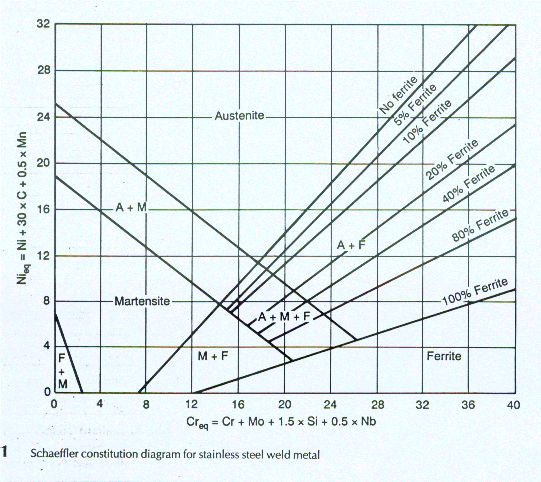
\includegraphics[width=.9\linewidth]{chapters/austenitic_steels_in_nuclear/plots/fecrschaeffler.png}
    \caption{Steel Cr-Ni Schaeffler Diagram}
    \label{fig:FeCrNiSchaeffler}
\end{minipage}
\begin{minipage}{.46\textwidth}
\centering
  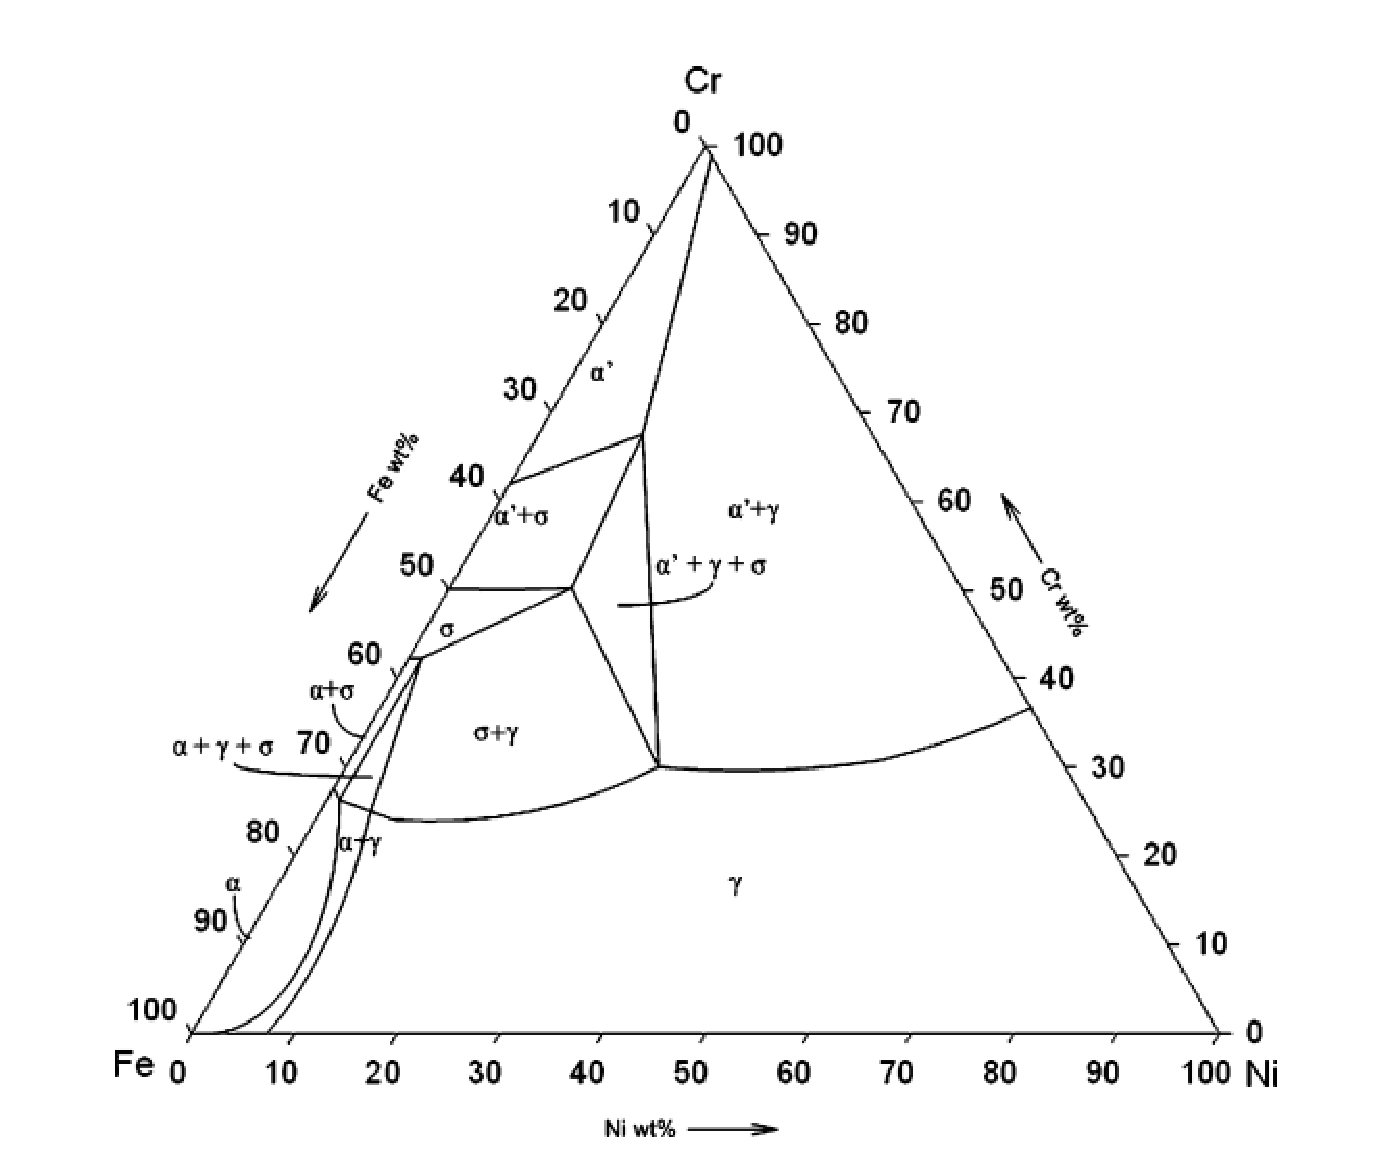
\includegraphics[width=.9\linewidth]{chapters/austenitic_steels_in_nuclear/plots/FeCrNi}
  \caption{Iron-Chromium-Nickel Phase Diagram\cite{fenicrternaryphase}}
  \label{fig:FeCrNi-PhaseDiagram}
\end{minipage}
\begin{minipage}{.05\textwidth}
\end{minipage}
\end{figure}


\subsubsection{Ferritic Stainless Steel}


\begin{figure}[ht]
\begin{tikzpicture}[scale=0.40]
\printtikzcrystalbcc{}
\end{tikzpicture} 
\caption{\acrshort{bcc} structure of ferritic stainless steel}
\label{fig:steelbcc}
\end{figure} 

At room temperatures and pressures, Fe exists in the alpha phase, which is a \acrshort{bcc} crystal.  It is energetically favourable for the magnetic moments of the Fe atoms to align with one another ferromagnetically.  Ferritic stainless steels also have the natural alpha phase crystal structure of pure Fe at room temperature which is \acrshort{bcc} (fig \ref{fig:steelbcc}).  These steels are magnetic and may be hardened by cold working.  They are less corrosion resistant than austenitic stainless steels.  Two common examples of this grade of steel are \acrlong{asme} codes 405 and 430.



\subsubsection{Austenitic Stainless Steel}

\begin{figure}[ht]
\begin{tikzpicture}[scale=0.40]
\printtikzcrystalfcc{}
\end{tikzpicture} 
\caption{\acrshort{fcc} structure of austenitic stainless steel}
\label{fig:steelfcc}
\end{figure} 

Austenite is a \acrshort{fcc} \gls{allotrope} of Fe (fig \ref{fig:steelfcc}), and austenitic stainless steels are useful in many applications, including a structural material for nuclear plant components, due to their resistance to corrosion.  In addition to 10.5 wt\% or more Cr they require an austenite stabilising element such as carbon and/or nickel to be added.  

Two examples of such steels are \acrshort{asme} codes 304 and 316.  Both have a high Cr content, in the region of 18-20\%, which is in excess of the minimum passive film requirement of around 10-11\%.  The natural structure of such an Fe Cr alloy would be \acrshort{bcc}, however 304 and 316 Steels contain Nickel (approximately 8\% and 10\% respectively) which is an austenite stabiliser, and this is responsible for the \acrshort{fcc} structure of the steel.  The 316 grade contains a minimum of 2\% Mo to improve its resistance to corrosion.

Ferritic and martensitic have a better resistance to thermal or swelling shock than austenitic \cite{bccfenimodel}, but the corrosion resistance of austenitic steels is a deciding factor when choosing a steel for an application where corrosion resistance is important.



\subsubsection{Martensitic Stainless Steel}

Martensitic stainless steels have a \acrshort{fcc} structure at high temperature, but when heat treated take on a \acrshort{bcc}  structure.  This allows martensitic, unlike austenitic and ferritic, to be hardened by heat treatment.  These steels are magnetic, they contain more than 10.5\% Cr but have a much lower Ni than austenitic grades, if any.  They are corrosion resistant, but the corrosion resistance of austenitic steel is typically better.  Two examples of such steels are ASME codes 410 and 431.  A comparison of properties between common grades of each steel are detailed in table \ref{table:steelproperties}. 


\begin{table}[h]
\begin{center}
\begin{tabular}{c c c c c c c}
\hline\hline
Grade & Code & \acrshort{hrb} & \Gls{proofstrength} (MPa) & UTS (MPa) & Density ($kgm^3$) & E (GPa) \\
\hline\hline
Austenitic      & 304 & 80 & 230 & 540-750  & 7900 & 200 \\
Austenitic      & 316 & 79 & 240 & 530-680  & 8000 & 200 \\
Ferritic        & 405 & 75 & 250 & 400-600  & 7700 & 220 \\
Ferritic        & 430 & 85 & 280 & 450-600  & 7700 & 220 \\
Duplex          & 255 & 32 & 550 & 750-1000 & 7800 & 200 \\
Martensitic     & 410 & 90 & 205 & 600      & 7700 & 215 \\
Martensitic     & 420 & 95 & 345 & 700      & 7700 & 215 \\
\hline\hline
\end{tabular}
\end{center}
\caption{Common grades of ferritic, austenitic, duplex and martensitic stainless steel and their properties.  Hardness using the \acrshort{hrb}, \gls{ultimatetensilestrength} (UTS) and \Gls{youngsmodulus} E.}
\label{table:steelproperties}
\end{table}





%%%%%%%%%%%%%%%%%%%%%%%%%%%%%%%%%%%%%%%%%%%%%%%%%%%%%%%%%%%%%%%%%%%%%%%%%%%%%%%%%%%%%%%%%%%%%%%%%%%%%%%%%%
%%
%%  Austenitic Steels
%%
%%%%%%%%%%%%%%%%%%%%%%%%%%%%%%%%%%%%%%%%%%%%%%%%%%%%%%%%%%%%%%%%%%%%%%%%%%%%%%%%%%%%%%%%%%%%%%%%%%%%%%%%%%



\section[Use In Reactors]{Austenitic Steels in Nuclear Reactors}

\subsection{The Use of Austenintic Steels in Reactors}

Due to their excellent strength and corrosion resistance, austenitic steels have been widely used in nuclear reactors.  The cheaper to manufacture \gls{304SS} and more corrosion resistant \gls{316SS} have been particularly popular choices of steel.  There are drawbacks, when compared to other alloys including ferritic and martensitic steels, and two in particular are \acrshort{igscc} and swelling.



\subsection{Atom Damage Cascades}

Fission fragments carry away the majority of the energy released during fission, with an approximate energy of 170MeV per 235U fission event.  The fragments are large and have a highly charged positive nucleus that stops rapidly due to the Coulomb interaction with the nuclei of surrounding atoms.  Electrons released by beta decay travel a greater distance; they lose energy by interacting with electrons, but may also knock atoms out of place.  Neutrons travel further still and lose energy by interacting directly with the nuclei of the surrounding material.

When an incoming projectile hits an atom (the \acrfull{pka}), it is knocked out of its place and loses energy by colliding with other atoms and to the electrons in the metal.  Depending on the energy of the \acrshort{pka}, this causes a damage cascade.  Atoms knocked out of their regular position in the crystal lattice leave vacancies behind.  The displaced atoms either recombine with vacancies, become interstitial atoms or diffuse to defect sinks.  A number of complex problems arise as a result of this damage, and this can take many years and high damage doses to appear.


\subsection{Damage Rates}
\FloatBarrier

The safety of a Nuclear reactor is the primary concern; it must generate power, but it must be safe.  It must also be cost efficient.  \acrshort{gen2} \acrshort{pwr} fuel assembles were expected to withstand several DPA\cite{genIVstrucmat}.  In \acrshort{bwr}s the materials are designed to be irradiated by $10^{22} n/cm^2/s$, experiencing approximately 7 \acrshort{dpa} over the lifetime of the components\cite{lightwaterallenbusby}.  Components in \acrshort{pwr}s are irradiated by up to $10^{22} n cm^{-2} s^{-1}$, and are expected to operate up to an irradiation dose of 70 dpa\cite{lightwaterallenbusby}.  To remain cost efficient, components in \acrshort{gen4} reactors will be expected to operate safely up to even higher doses or irradiation damage (fig \ref{fig:genIVdpa}).  Components in sodium-cooled fast reactors will be expected to withstand up to 200 DPA over their lifetime to meet the requirements of cost effectiveness and durability\cite{genIVstrucmat}.


\begin{figure}[h]
  \begin{center}
    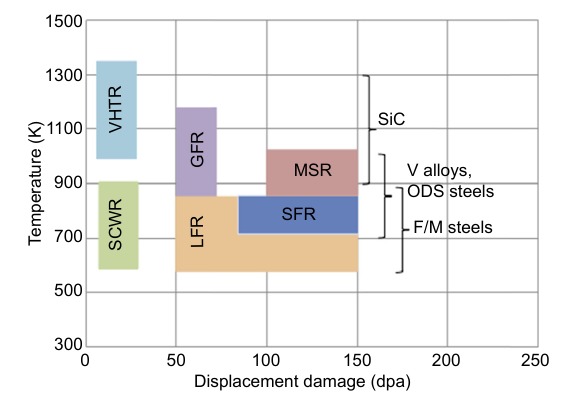
\includegraphics[scale=0.55]{chapters/austenitic_steels_in_nuclear/images/dpagenIV.png}
    \caption{Expected DPA during component life time and operating temperatures\cite{genIVstrucmat}}
    \label{fig:genIVdpa}
  \end{center}
\end{figure}
\FloatBarrier

Neutrons released during the fission of U235 range from 0 to 14 MeV (fig \ref{fig:neutronfissionspectra}), and the energy transferred to a target atom depends on the scattering angle of the neutron and the mass of the target nucleus.  

\begin{equation}
\begin{split}
\alpha = (\frac{m_N-1}{m_N+1})^2 \\
E_N = E_n \left(1 - \frac{(1+\alpha) + (1 - \alpha) cos \theta_C}{2}\right)
\end{split}
\label{eq:eqNeutronEnergyTransfer}
\end{equation}

\begin{figure}
\centering
\begin{minipage}{.46\textwidth}
\centering
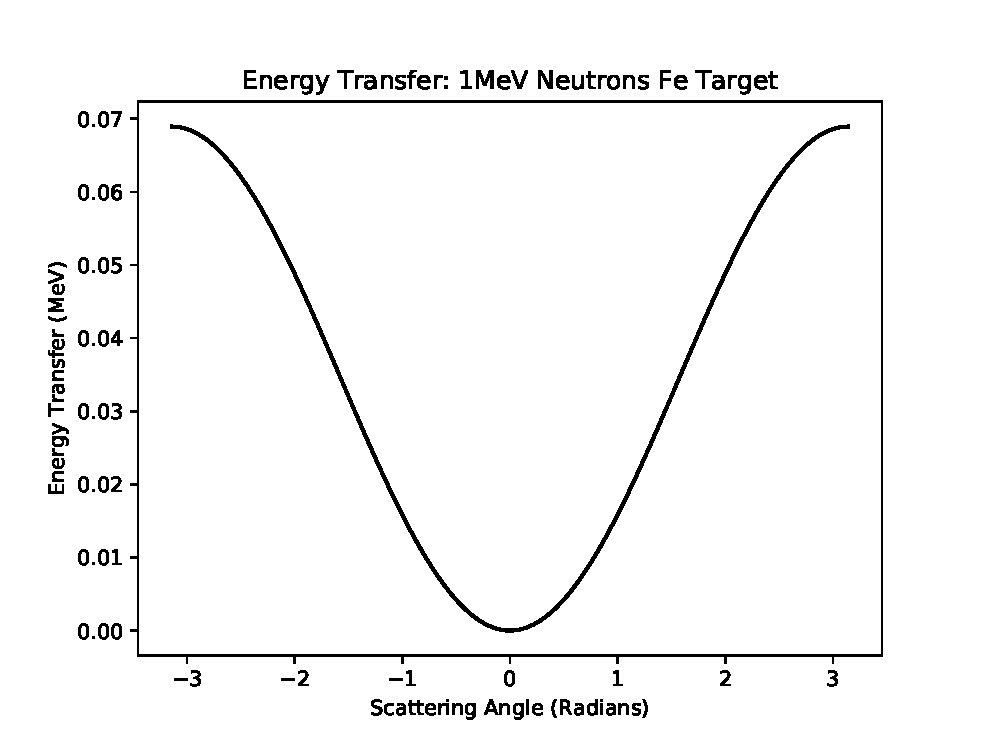
\includegraphics[width=.9\linewidth]{chapters/austenitic_steels_in_nuclear/plots/scattering_angle.eps}
\caption{Scattering angle probability of neutrons}
\label{fig:scatteringangle}
\end{minipage}
\begin{minipage}{.05\textwidth}
\end{minipage}
\begin{minipage}{.46\textwidth}
\centering
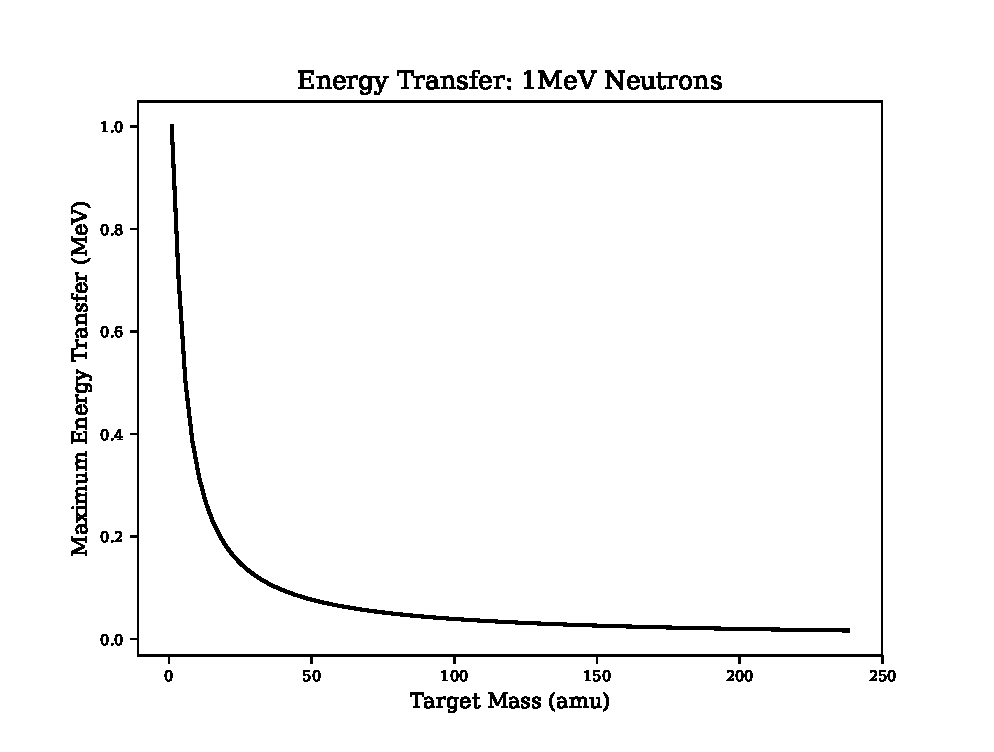
\includegraphics[width=.9\linewidth]{chapters/austenitic_steels_in_nuclear/plots/nuclei_mass.eps}
\caption{Energy transfer as a from a neutron dependant on target mass}
\label{fig:energytransfer}
\end{minipage}
\end{figure}

In a collision, the amount of energy transferred to a target atom will depend on both the scattering angle of neutron recoiling from the target and the mass of the target nucleus.  If the neutron does not change direction, a small amount of energy will be transferred, but if it bounces back at 180 degrees it will transfer the maximum amount of energy.  A neutron will lose more energy per collision with light atoms (hydrogen, helium, carbon), but much less energy per collision with larger atoms (iron, molybdenum, lead).

\begin{figure}[h]
  \begin{center}
    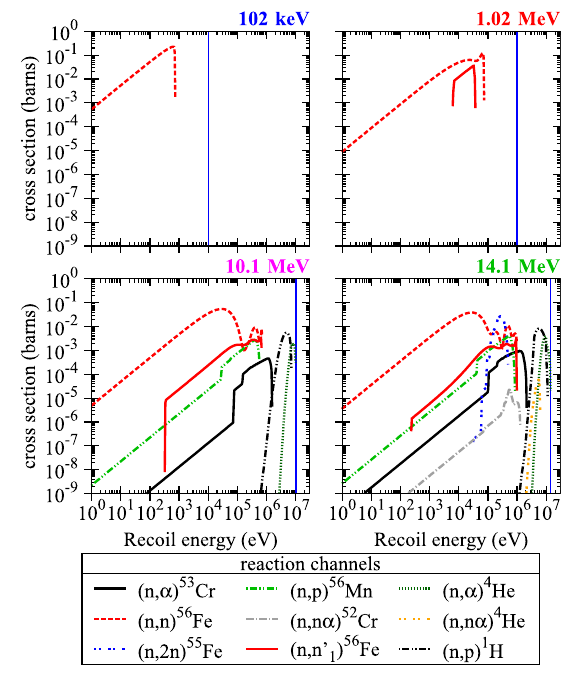
\includegraphics[width=.65\linewidth]{chapters/austenitic_steels_in_nuclear/images/neutronrecoils.png}
    \caption{Recoil energies for neutrons at 102keV, 1.02MeV, 10.1MeV and 14.1MeV\cite{pkaenergyspectra}}
    \label{fig:ferecoilchannels}
  \end{center}
\end{figure}
\FloatBarrier


The energy of Fe \acrshort{pka}s as a result of neutron irradiation has been calculated for an Fe target\cite{pkaenergyspectra} (fig. \ref{fig:neutronironrecoil}), and those created by 1MeV neutrons may have an energy up to 100keV.  As nuclear reactions are also possible between the neutrons and the target nuclei, there is an inelastic $(n,n) {}^{56}Fe$ channel as well as other elastic scattering channels where the post collision particles are different to the pre collision particles (fig. \ref{fig:ferecoilchannels}).






\FloatBarrier

\subsection{Swelling}

Swelling results from damage to the crystalline structure of the metal, and is formed through small voids being created in the crystal.  As vacancies are created by radiation damage, they precipitate into small voids.  The temperature range for such swelling is primarily from $670K$ to $870K$.

Materials have been known to swell to a 100\% increase in their original volume at these intermediate temperatures under irradiation\cite{wasstrucaustenitic}.  Swelling is sensitive to the total damage amount, the temperature and composition of the alloy.  An increase in Ni decreases swelling as does the addition of Zr.  Small amounts of \Gls{P} and Mo (0.02\% and 0.5-1.0\% respectively) cause the swelling of the alloy to increase, however higher concentrations of either cause swelling to decrease\cite{swellingris}.

As a component swells its properties change.  By definition the volume changes, but so does the elastic moduli.  Not only this, but the swollen component may stress itself and surrounding components, and this may lead to \acrshort{scc}.

In the \acrshort{ebr}-II structural \gls{304SS} was irradiated to 20\acrshort{dpa}.  At a temperature of approximately $650K$ the steel's volume increased by 2\% due to swelling\cite{radisandvoid}.  With components in future reactors expected to withstand ten times this damage, swelling is a concern.  However, increased temperatures and a careful balance in the composition of future alloys will help to reduce this.



\FloatBarrier


\subsection{Radiation Induced Segregation}

The diffusion of atoms within an alloy has an impact on the characteristics of the metal \cite{nickeldiffusion}.  When radiation causes point defects, these interstitials also diffuse parallel to thermal solute diffusion.  At low temperatures, the atoms are unable to diffuse at an appreciable rate; the mobility of vacancies are low\cite{gswas} and there are an excess of vacancies due to radiation damage, and this leads to recombination of defects.  At high temperatures, there is a higher concentration of thermal defects\cite{lightwaterallenbusby}.  This increases the defect recombination rate and reduces migration of defects to sinks, such as grain boundaries.

The melting temperature range of 304 and 316 stainless steel are approximatelyh 1695-1722K and 1644-1672K respectively.  \acrshort{gen2} reactors, such as Sizewell B, have an operating temperature of several hundred degrees centigrade.  The inlet temperature for the Sizewell B PWR reactor is 566K\cite{sizewellbtemp} and the outlet temperature is 597K\cite{sizewellbtemp}.  Operating at approximately 35\% the melting point of the steel this is, unfortunately, a good temperature for \acrfull{ris} to occur.

The \acrfull{ke} concerns the diffusion of one material into another and vice versa at an interface.  In the original experiment performed by Kirkendall and Smigelskas, brass (\Gls{Cu} and Zn) was sandwiched between \Gls{Cu} and left at a temperature of over 1050K for almost two months.  Using Mo as a marker, it was discovered that Zn diffused out of the brass faster than the copper diffused into the brass.  The flux of atoms results in a flux defects and a shrink in volume of brass\cite{gswasike}.

The \acrfull{ike} is driven by an external force, such as irradiation.  Irradiation of the material causes a flux of defects and, inverse to the \acrshort{ke}, this causes a flux of atoms.  For an austenitic stainless steel the diffusion coefficients in order of size are $D_{Cr} > D_{Fe} > D_{Ni}$\cite{risfecrni}, so Cr will diffuse away from grain boundaries and other sinks, followed by Fe.  As Ni is slowest to diffuse, this will be enriched.  An additional mechanism that is thought to contribute to \acrshort{ris} is interstitial flux where undersized atoms as interstitials are preferential\cite{risfecrni}.

\begin{figure}
\centering
\begin{minipage}{.46\textwidth}
\centering
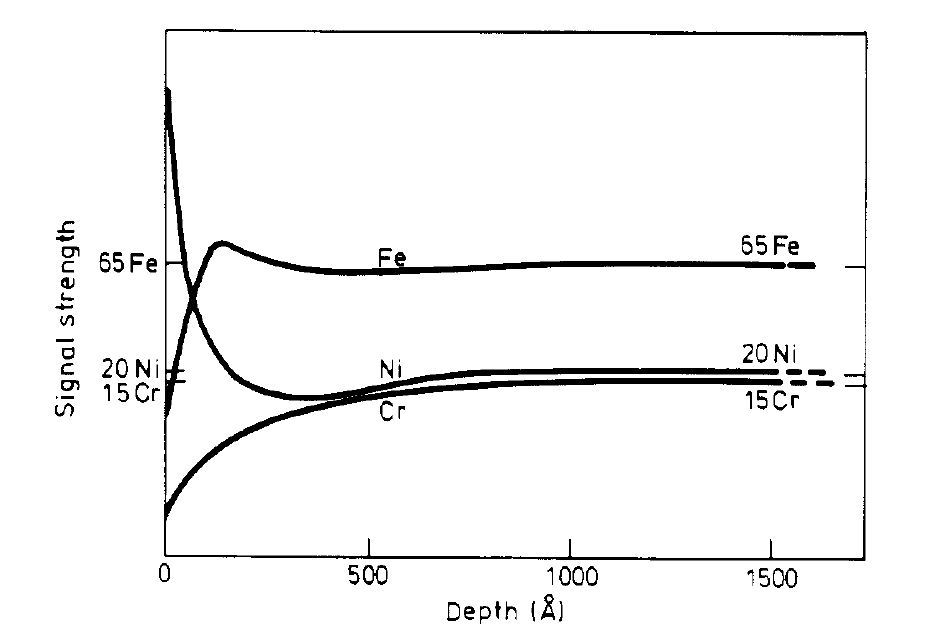
\includegraphics[width=.9\linewidth]{chapters/austenitic_steels_in_nuclear/images/marwickfecrniseg1.png}
\caption{Depletion of cr, fe and enrichment of ni at the surface\cite{johnstonris}}
\label{fig:johnstonris}
\end{minipage}
\begin{minipage}{.05\textwidth}
\end{minipage}
\begin{minipage}{.46\textwidth}
\centering
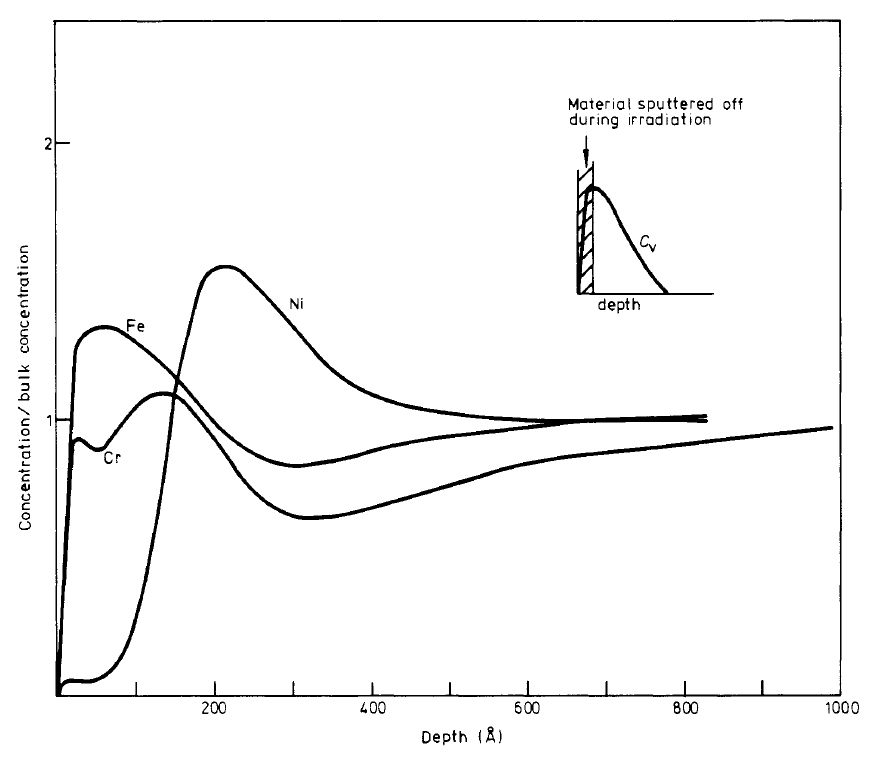
\includegraphics[width=.9\linewidth]{chapters/austenitic_steels_in_nuclear/images/marwickfecrniseg2.png}
\caption{Concentration profile after 46\acrshort{dpa} irradiation with 75 keV Ni ions\cite{marwickris}}
\label{fig:marwickris}
\end{minipage}
\end{figure}

\FloatBarrier

Experimental work by Johnston et al irradiated steel, containing 15\% Cr and 20\% Ni, with 4MeV Ni ions.  It was irradiated to a damage dose of 8\acrshort{dpa} at $950K$.  Some material will have been sputtered from the surface, but in the remaining material Cr, and Fe, were depleted.  Ni, however, was enriched (fig. \ref{fig:johnstonris}).

In work by Marwick a similar alloy with 14\% Cr and 15\% Ni was irradiated to a much higher dose of 46 \acrshort{dpa} with lower energy 75KeV Ni ions.  In this instance the damage occurs in a much thinner layer of the surface that was approximately 30nm thick (fig. \ref{fig:marwickris}).  Conversely to Johnston et al, in this thin layer there is a depletion of Ni and an enrichment of Cr in the first 20nm or so.  However, between approximately 25nm and 60nm there is a similar depletion of Fe and Cr as well as an enrichment of Ni.


\begin{figure}[h]
  \begin{center}
    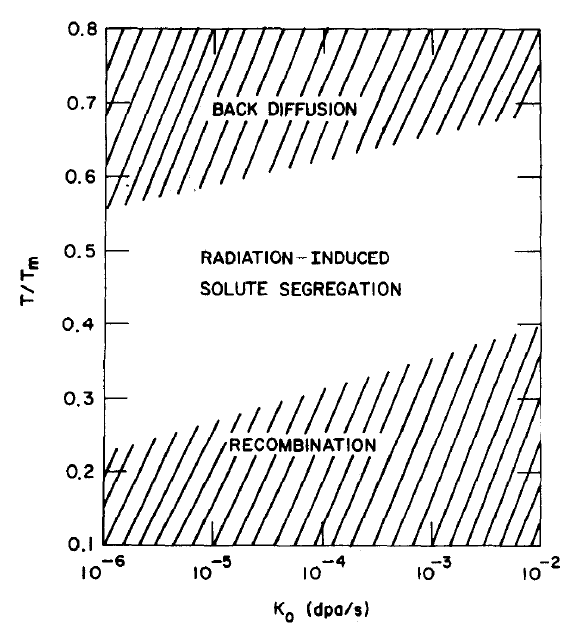
\includegraphics[width=.5\linewidth]{chapters/austenitic_steels_in_nuclear/images/okamoto_rehn_temp_ris.png}
    \caption{Temperature and \acrshort{dpa} dependence of \acrshort{ris}\cite{risokamoto}}
    \label{fig:ristemperature}
  \end{center}
\end{figure}

The underlying mechanisms of \acrshort{ris} are dependent on both the temperature (relative to the melting point of the material) and the amount of damage (fig. \ref{fig:ristemperature}).  The result of \acrshort{ris} is a breakdown in the passive protection of Cr, which leads to \acrshort{igscc} under the correct conditions.


\FloatBarrier

%\begin{figure}[h]
%  \begin{center}
%    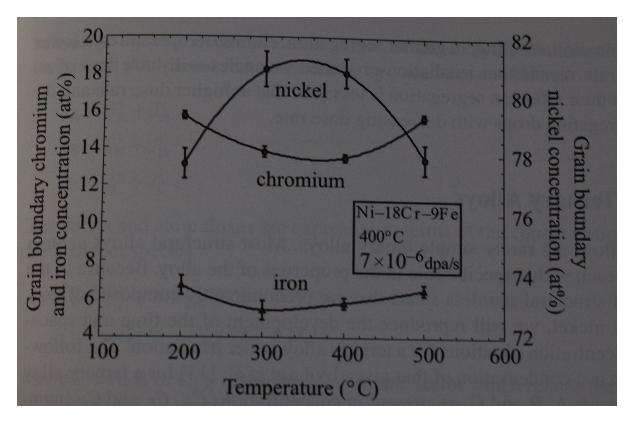
\includegraphics[width=.65\linewidth]{chapters/austenitic_steels_in_nuclear/plots/nicrfeseg.eps}
%    \caption{Grain boundary concentrations at $200^{\circ}C$ to $500^{\circ}C$}
%    \label{graph:grainboundaryconc}
%  \end{center}
%\end{figure}

%\begin{figure}[h]
%  \begin{center}
%    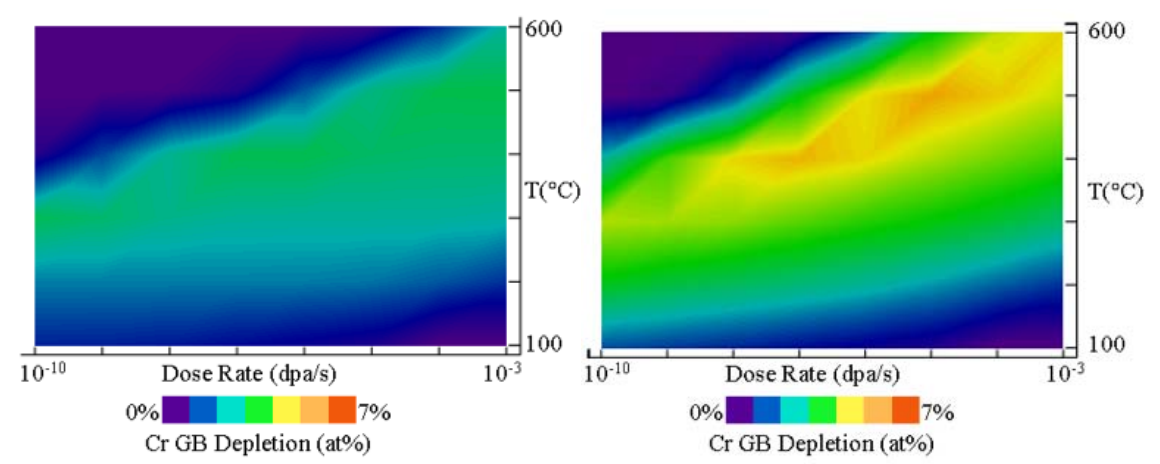
\includegraphics[width=.65\linewidth]{chapters/austenitic_steels_in_nuclear/images/crseg.png}
%    \caption{Chromium grain boundary depletion}
%    \label{graph:crgbdepletion}
%  \end{center}
%\end{figure}



\FloatBarrier





%%%%%%%%%%%%%%%%%%%%%%%%%%%%%%%%%%%%%%%%%%%%%%%%%%%%%%%%%%%%%%%%%%%%%%%%%%%%%%%%%%%%%%%%%%%%%%%%%%%%%%%%%%
%%
%%  Corrosion Resistance
%%
%%%%%%%%%%%%%%%%%%%%%%%%%%%%%%%%%%%%%%%%%%%%%%%%%%%%%%%%%%%%%%%%%%%%%%%%%%%%%%%%%%%%%%%%%%%%%%%%%%%%%%%%%%


\section[Corrosion Resistance]{Corrosion Resistance of Austenitic Stainless Steels}

\subsection{Passive Film Protection of Chromium}

The addition of Cr improves the resistance of stainless steel to corrosion by orders of magnitude.  A very thin passive oxide layer, 20-30 angstroms in width, forms when the surface is exposed to an environment containing oxygen.  The protective layer is self repairing and, if the surface is damaged, the oxide layer reforms in the presence of oxygen.

When the steel is in an environment containing oxygen, electrons within the metal tunnel through the surface.  As an oxidizing agent, the nearby oxygen atoms readily accept the electrons.  A strong electric field forms between positive ions within in the metal and the negatively charged oxygen atoms \cite{medicalmetals133}.  

Fe at the surface of the forming oxide layer is preferentially dissolved away over Cr \cite{kirchheimcc} and Cr ions within the oxide layer have a lower mobility than Fe ions \cite{kirchheimpassive}.  Ni remains in place within the alloy, and this leads to an enrichment of chromium oxide in the passive layer.  Once the layer is thick enough to reduce the electric field across it, the formation of the layer stops.  As mentioned previously, this is at a layer thickness of 2-3nm for stainless steel.

The $\text{Cr}_{2}\text{O}_{3}$ layer may be formed by heating the steel to $770K$\cite{propaustenitic}.  However, at higher temperatures, the steel begins to lose its protective layer due to \gls{sensitization}.


\subsection{\Gls{sensitization} and Passive Film Removal}

Steel by definition is Fe alloyed with varying small percentages of C.  C changes the property of the alloy, and one example of this is an increase in hardness over pure Fe.  At elevated temperatures, 670K to 1020K, the added Cr within the steel forms precipitates of Fe-Cr carbides $(\text{Fe}\text{Cr})_{23} C_{6}$ at the grain boundaries, reducing the percentage of Cr at the grain boundary and removing the layer of passive protection.

\begin{figure}
\centering
\begin{minipage}{.46\textwidth}
\centering
  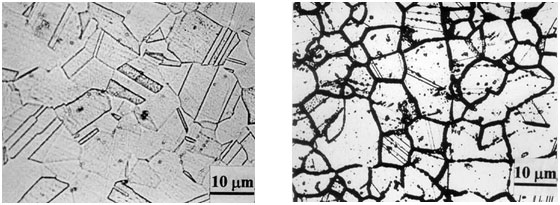
\includegraphics[width=.9\linewidth]{chapters/austenitic_steels_in_nuclear/images/alloy-sensitization.jpg}
  \caption{Formation of chromium precipitates at the grain boundary \cite{rolledalloys}}
  \label{fig:alloysensitization1}
\end{minipage}
\begin{minipage}{.05\textwidth}
\end{minipage}
\begin{minipage}{.46\textwidth}
\centering
  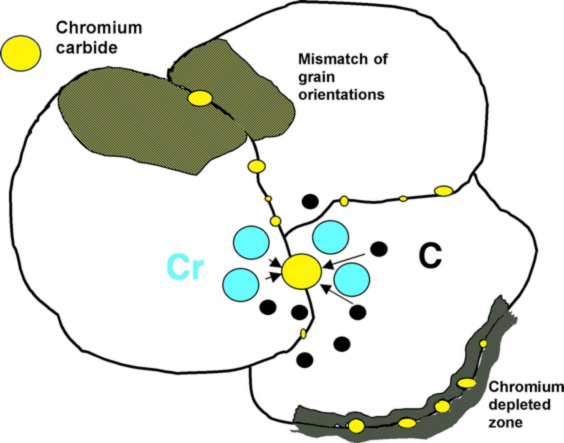
\includegraphics[width=.9\linewidth]{chapters/austenitic_steels_in_nuclear/images/Intergranular-corrosion__figure2.jpg}
  \caption{Sensitization of an alloy: chromium carbide precipitation \cite{ssina}}
  \label{fig:alloysensitization2}
\end{minipage}
\end{figure}

The sensitization of the steel can be reversed.  By heating the steel further, to approximately 1,320K to 1,420K, the steel is solution annealed dissolving the carbides back into the steel.



\subsection{Addition of Molybdenum}

A common austenitic stainless steel is \gls{304SS} and this relies heavily on the passive film due to a high content of Cr, ranging from 17.5\% to 20\% for grades 304, 304L and 304H.  A similar stainless steel, 316, has slightly less Cr, slightly more Ni and 2-3\% Mo, an element not present in 304 stainless steel.

Pure Mo has a \acrshort{bcc} crystal structure, and it is a ferrite former.  However, high proportions of austenite former such as Ni and N force 316 stainless steel to keep its \acrshort{fcc} structure despite the addition of Mo.  Adding it to austenitic steels improves their strength and resistance to creep at high temperatures.  

Steels such as \gls{316SS} are known to have better corrosion resistance in chloride rich environments.  Where at least 2\% Mo has been added it improves resistance to pitting and crevice corrosion resistance\cite{corrosionmo}.  The mechanism by which Mo helps to protect against corrosion is still unclear.  It is possible the addition helps to reduce the breakdown of the passive film protecting the steel, but it may also be the case that Mo promotes the repair of the passive film \cite{moprotection}.














%%%%%%%%%%%%%%%%%%%%%%%%%%%%%%%%%%%%%%%%%%%%%%%%%%%%%%%%%%%%%%%%%%%%%%%%%%%%%%%%%%%%%%%%%%%%%%%%%%%%%%%%%%
%%
%%  Intergranular Stress Corrosion Cracking
%%
%%%%%%%%%%%%%%%%%%%%%%%%%%%%%%%%%%%%%%%%%%%%%%%%%%%%%%%%%%%%%%%%%%%%%%%%%%%%%%%%%%%%%%%%%%%%%%%%%%%%%%%%%%




\section[IASCC]{Irradiation Assisted Stress Corrosion Cracking}

\FloatBarrier

Damage due to irradiation was first identified in high stress stainless steel components in a reactor, such as bolts, springs, and fuel elements\cite{gswasiascc}\cite{iascckenikjonesbell}, and later being found in lower stress austenitic stainless steel components\cite{iascckenikjonesbell}.

\begin{figure}
  \begin{center}
    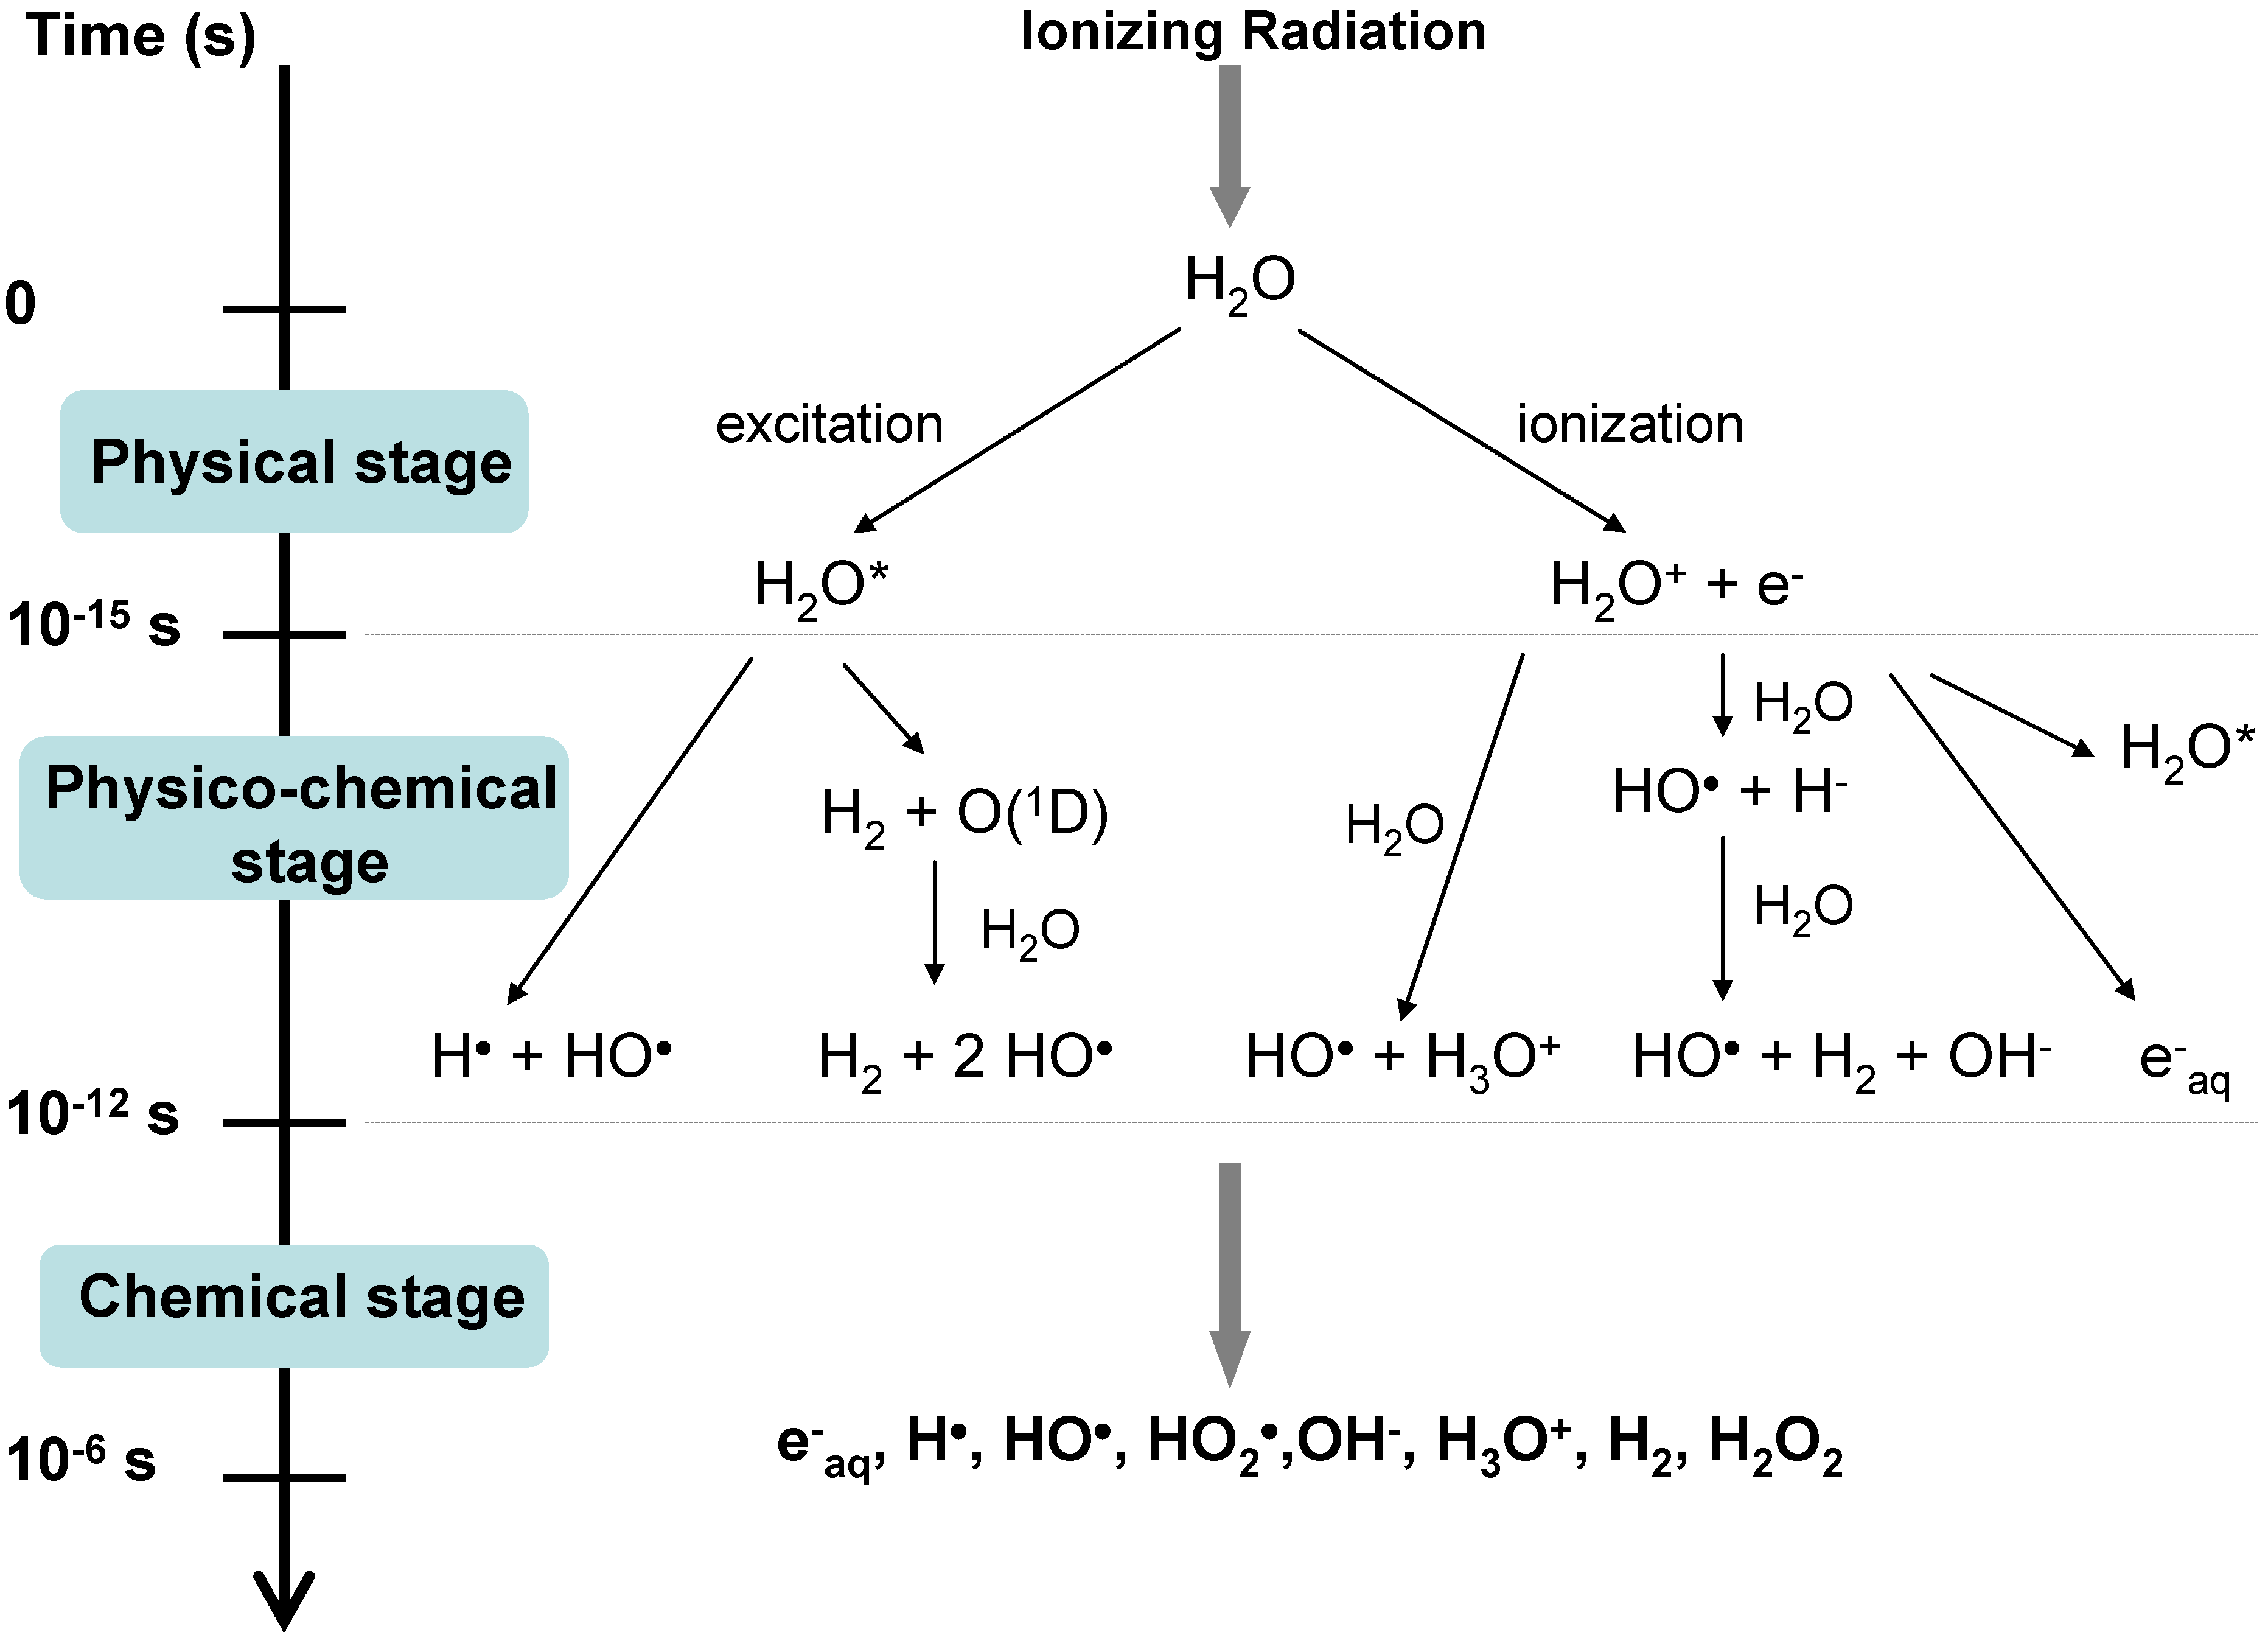
\includegraphics[width=.5\linewidth]{chapters/austenitic_steels_in_nuclear/images/water_radiolysis.png}
    \caption{Changing water chemistry: radiolysis of water\cite{waterradiolysis}}
    \label{fig:radiolysisofwater}
  \end{center}
\end{figure}

Irradiation of water causes the radiolysis of water, changing the chemistry of water and creating hydrogen, radicals and other ions that increase the corrosiveness of the environment (fig \ref{fig:radiolysisofwater}).  The radiation also damages the material directly, changing its properties.  A form of \acrshort{iascc} to which high nickel alloys, including austenitic steels, are particularly susceptible to is \acrlong{igscc}.



\section[IGSCC]{Inter Granular Stress Corrosion Cracking}

Stress corrosion cracking may be trans granular (through the grains) or inter granular, at the grain boundary.  \acrshort{igscc} is a particularly prominent failure mechanism for austenitic stainless steels.  For \acrshort{igscc} to occur, there must be a material that is susceptible to this form of cracking, an environment that is corrosive to the material as well as stress (fig. \ref{fig:igsccrequirements}).  

\begin{figure}
  \begin{center}
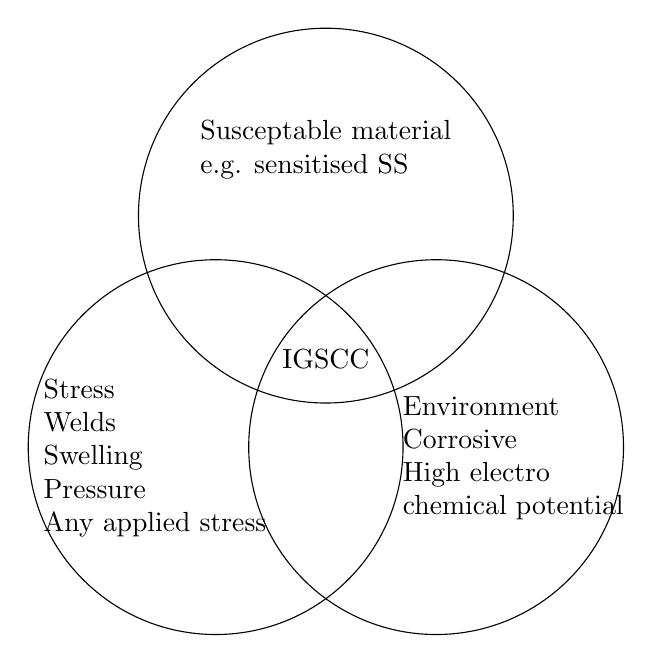
\begin{tikzpicture}[scale=0.70]
\draw (4.5,5.0) circle [radius=3.4];
\draw (2.5,0.8) circle [radius=3.4];
\draw (6.5,0.8) circle [radius=3.4];
\node[align=left] at (4.5, 2.4) {IGSCC};
\node[align=left] at (1.4,0.6) {Stress\\Welds\\Swelling\\Pressure\\Any applied stress};
\node[align=left] at (4.5, 6.2) {Susceptable material \\ e.g. sensitised SS};
\node[align=left] at (7.9,0.6) {Environment\\ Corrosive\\ High electro \\chemical potential};
\end{tikzpicture}
\caption{Three requirements for \acrshort{igscc} to occur}
\label{fig:igsccrequirements}
\end{center}
\end{figure}

Stress may come from a high pressure environment or residual stresses due to welding.  In a nuclear reactor the atomic structure may be under stress due to damage caused by neutrons passing through the steel, or due to the swelling of the steel on the macroscopic scale.  If Cr is depleted at the grain boundary, protection to corrosion due to the passive layer is lost.  This, coupled with the knowledge that austenitic stainless steels are susceptible to \acrshort{igscc}, completes the three requirements and, over time, components of this material in these conditions will eventually fail to \acrshort{igscc}.

\acrshort{igscc} has not only been a defect in stainless steel.  High Ni content alloys, such as Alloy 600 (Inconel:  Ni-72, Cr-17, Fe-10),  have been known to suffer from \acrshort{igscc} since the very early days of nuclear energy, in particular with the prototype S1W reactor, prototype for the first nuclear powered submarine, the USS Nautilus.

\begin{figure}
  \begin{center}
    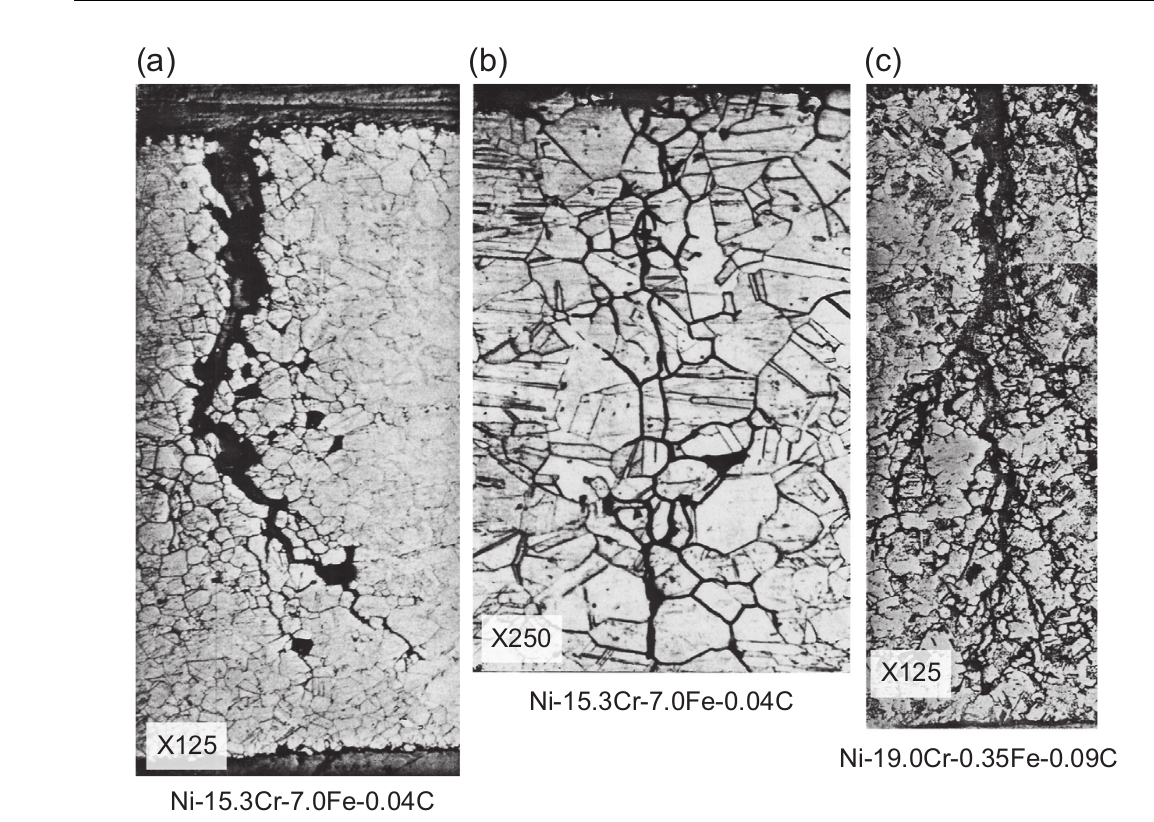
\includegraphics[width=7.0cm]{chapters/austenitic_steels_in_nuclear/images/igscc_nickel_alloy600.png}
    \caption{Inter Granular Stress Corrosion Cracking in Nickel Alloy\cite{staehlecoriou}}
    \label{image:igsccni}
  \end{center}
\end{figure}

After the war, there was a drive to develop a nuclear powered navy for the US.  There are obvious benefits in replacing conventional power in vessels with nuclear, in particular for submarines.  This was pushed by Admiral Rickover and the route to building the USS Nautilus began.  A number of available Fe-Cr-Ni alloys were considered for the construction of the reactor (fig. \ref{fig:fecrnialloys}).

\begin{figure}
\centering
\begin{minipage}{.46\textwidth}
\centering
    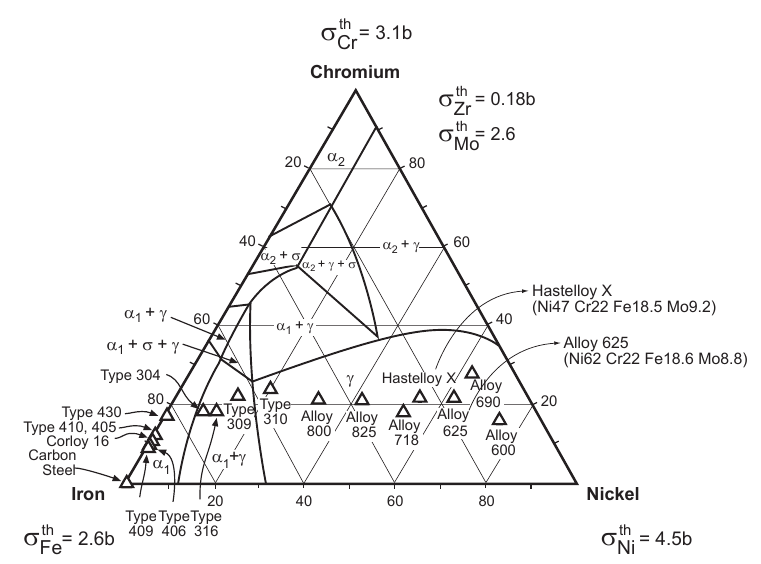
\includegraphics[width=.8\linewidth]{chapters/austenitic_steels_in_nuclear/images/fecrnialloys.png}
    \caption{Alloy choices for early LWRs}
    \label{fig:fecrnialloys}
\end{minipage}
\begin{minipage}{.05\textwidth}
\end{minipage}
\begin{minipage}{.46\textwidth}
\centering
    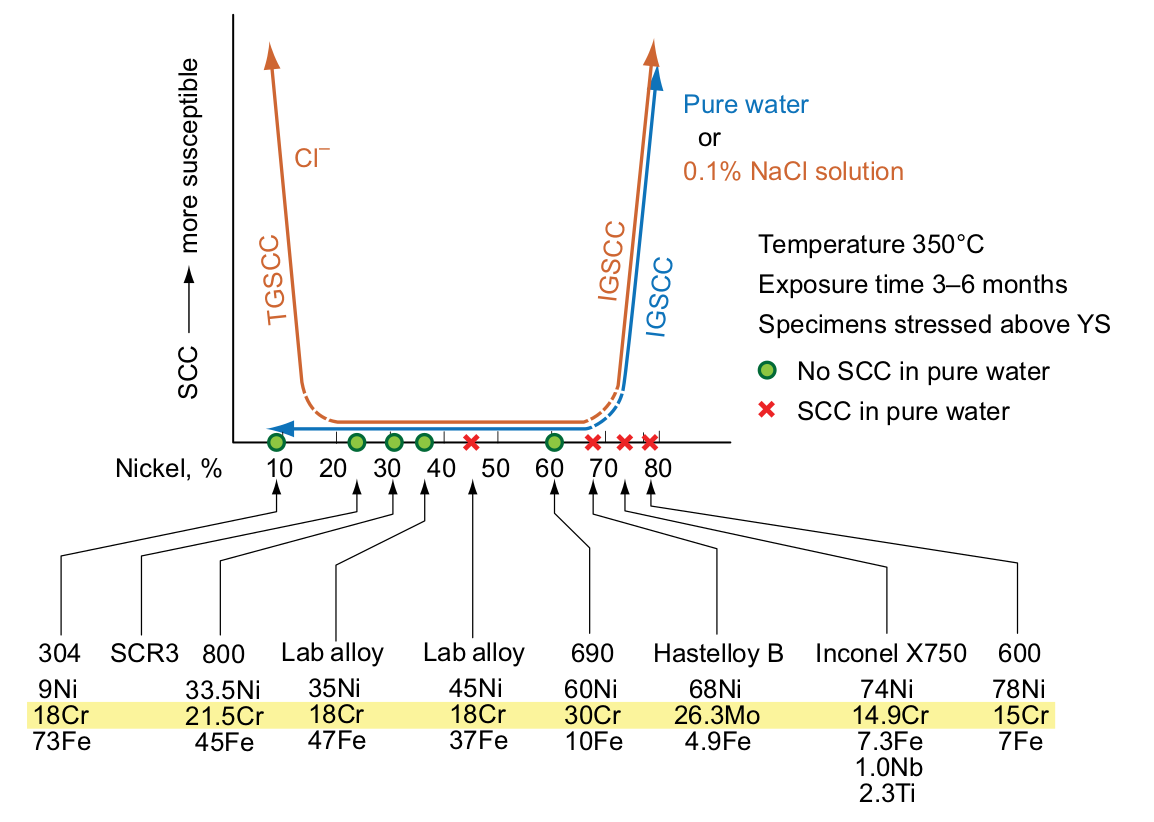
\includegraphics[width=.8\linewidth]{chapters/austenitic_steels_in_nuclear/images/tgscc_igscc_vs_nickel.png}
    \caption{Nickel, IGSCC and TGSCC}
    \label{fig:nitgsccigscc}
\end{minipage}
\end{figure}

Prototypes developed for the USS Nautilus experienced stress corrosion cracking in the Inconel Alloy 600 components.  H. Coriou replicated this damage to Inconel in the laboratory, holding a sample at $620K$ in deoxygenated water for 3 months\cite{staehlecoriou}.  Further studies showed that \acrshort{igscc} became a particular issue to alloys with a high Ni content in pure water, commencing with a content of approximately 70\% Ni.  In a weak salt water solution (0.1\% NaCl) \acrshort{igscc} occurred as with the same alloy in pure water, but \acrshort{tgscc} occurred in similar alloys with a low Ni content (less that 15\%) (fig. \ref{fig:nitgsccigscc}).


\FloatBarrier

\subsection{IGSCC in Light Water Reactors}

In \acrshort{lwr}s a major factor in corrosion of components is the water chemistry and \acrlong{ecp} that they operate in.  Higher levels of oxygen dissolved in the water leads to an increase in the corrosion potential\cite{wasstrucaustenitic}.  Other factors within \acrshort{lwr}s include depletion of Cr due to either heat treatment, welding or irradiation.

The primary circuit of a \acrshort{bwr} includes components such as a reactor pressure vessel, piping that leads out of the containment building, fuel and fuel assembly.  300 series steels, including 304 and 316, are used within the primary circuit, including the piping and control cod absorbers.  In \acrshort{bwr}s the purity of the water has been addressed, and the addition of hydrogen to the water has reduced cracking of components\cite{staehlecoriou}.  

Higher nickel content steels such as the 600 series alloys are used in \acrshort{pwr}s, and components that are made from these alloys include steam generators and pressure vessels.  In the AP-1000 design, the control rod drive mechanism at the reactor coolant pressure boundary are made from 304, 304L, 304LN, 316, 316L and 316LN steel.  Higher nickel content 690 is used for penetration into the pressure vessel\cite{ap1000dcd}.  As illustrated by Coriou's work in the 1950s and 1960s, higher nickel content steels are susceptible to \acrlong{scc}.

\FloatBarrier
\subsection{IGSCC and Advanced Gas-cooled Reactors}

The first generation of nuclear reactors in the UK were Magnox type reactors.  They used un enriched Uranium 0.7\% U235 as fuel which was contained within magnesium oxide cladding due to its low absorption cross section.  A major drawback was the relatively low operating temperature of $630K$.

Carnot's theorem shows that the maximum amount of energy from an engine is dependent on the difference between the hot and cold reservoirs (section \ref{section:carnottheorem}).  The ambient temperature of the power station will vary a small amount with the seasons.  The practical way to improve the maximum possible efficiency is to increase the engine (reactor) temperature.

\begin{equation}
\begin{split}
\eta_{max} = 1 - \frac{T_c}{T_h}
\text{where the temperature is measured in absolute units}
\end{split}
\end{equation}

\acrshort{agr}s were designed to run at much higher temperatures of $920K$.  By increasing the temperature, the maximum possible thermal efficiency was increased from just over 50 percent to almost 70 percent.  To withstand higher temperatures, the magnesium oxide cladding used in the earlier Magnox reactors was replaced with stainless steel.  To counteract the higher neutron absorption cross section of the cladding, the fuel was enriched up to 3.5\% $\text{U}^{235}$.

The cladding holds the fuel elements together and at the required location inside the reactor whilst it is consumed in the reactor.  The cladding also performs several functions once the fuel has been spent.  It holds the fuel elements together and acts as a primary containment for the spent fuel\cite{agrfuelstorage}.

During its lifetime as a fuel element within the reactor, the cladding has been heated and irradiated.  By the process of \acrshort{ris} the Cr at the grain boundary can drop to 10\% concentration\cite{agrigscc}.  The C rich environment within the reactor, due to the $\text{CO}_{2}$ coolant, provides yet another mechanism to deplete Cr at the grain boundary by the formation of Fe-Cr carbides $(\text{Fe}\text{Cr})_{23} C_{6})$.  

This loss of protection at the grain boundary, stress due to the role of the component within the reactor, the changing environment due to radiation damage and the material's susceptibility lead to \acrshort{igscc}.




\FloatBarrier



\section[SS in Gen III+ and Gen IV]{Austenitic Stainless Steels in Gen III+ and Gen IV Reactors}

The AP1000 is an advanced \acrshort{pwr}.  As a Westinghouse reactor, the fuel cladding will be their trademarked Zirlo alloy.  Inconel will be used for the steam generator and heat exchanger with carbon steel used for the construction of the pressure vessel.  The control rod absobers, however, will be constructed from \gls{304SS}\cite{ap1000mat}.

Areva designed the EPR and this will use \gls{316SS} as the fuel cladding material.  It will also use the slightly less corrosion resistant \gls{304SS} (forged) in parts of the control rod drive mechanisms\cite{eprmat}.

The perforated upper core plate, between the reactor core and the inlet/outlet/control rod mechanisms, is also made from austenitic stainless steel.  The pressuriser is constructed from ferritic steel, but its internals are clad with austenitic stainless steel to protect the structure from the coolant.

\acrshort{gen4} designs also include the use of austenitic stainless steels.  Experimental fast reactors in many countries, including the US, UK, Japan, France, India and China have used either \gls{304SS}, \gls{316SS} or both in their construction.

Austenitic steels are more corrosion resistant than ferritic or martensitic steels.  The do expand more as a result of being irradiated, but they are stronger at higher temperatures.  Many of the \acrshort{gen4} reactors operate at much higher temperatures than existing reactors and the components will be expected to resist higher doses of radiation damage throughout their lifetime.

\acrshort{gfr}s are expected to use austenitic steels.  Due to their chemical compatibility with sodium they are also expected to be used in \acrshort{sfr}s.  As well as being used in the reactor core, these steels will also be used outside the core.  For example, \acrshort{sfr}s in France will use austenitic steels in the secondary circuit, primary pump, internal heat exchanger and more\cite{convsteelooc}.


\FloatBarrier



\section[Addition of PGMs]{The Addition of PGMs to Stainless Steel}

Water purity is a concern for light water reactors.  The fewer contaminants there are to begin with, the better.  Even so, the radiolysis of the purest water will still create a steady supply of corrosive molecules (fig. \ref{fig:radiolysisofwater}).  Adding hydrogen to the water reduces the \acrlong{ecp} of the water, but if too much is added it will combine with the radioactive nitrogen-16 created by the ${}^{16}O(n,p){}^{16}N$ reaction to form ${}^{16}NH_{3}$\cite{noblemetalchemical}.

Cathodic modification is a technique used to improve corrosion resistance, and one way to do this for stainless steel is to add small amounts of \acrfull{pgm}s\cite{potgieter1994}.  By adding such metals, the anodic reaction may be reduced.  \acrshort{pgm}s also act as a catalyst in the reduction and removal of $O_2$ and $H_2O_2$ from the water\cite{noblemetalchemical}.

The increased corrosion resistance is dependant upon the amount of \acrshort{pgm} added, but a higher percentage does not necessarily mean better protection.  This is important for two reasons, to find the optimum amount for the sake of corrosion resistance, and to keep the price down as the additions are so expensive, even in such small amounts.

\begin{figure}
\centering
\begin{minipage}{.44\textwidth}
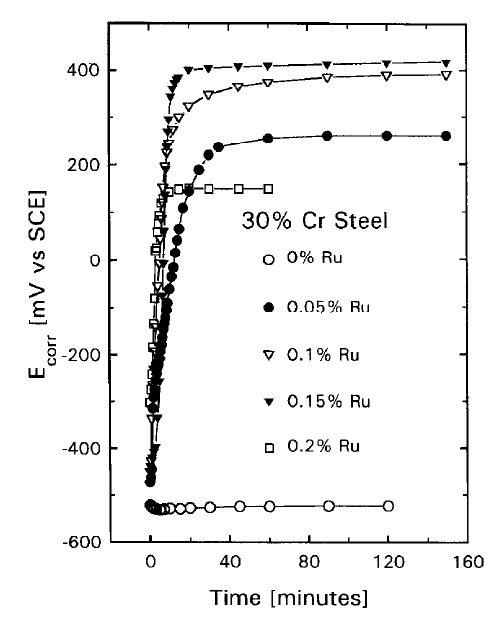
\includegraphics[width=.95\linewidth]{chapters/austenitic_steels_in_nuclear/images/fe30crru.png}
\end{minipage}
\begin{minipage}{.44\textwidth}
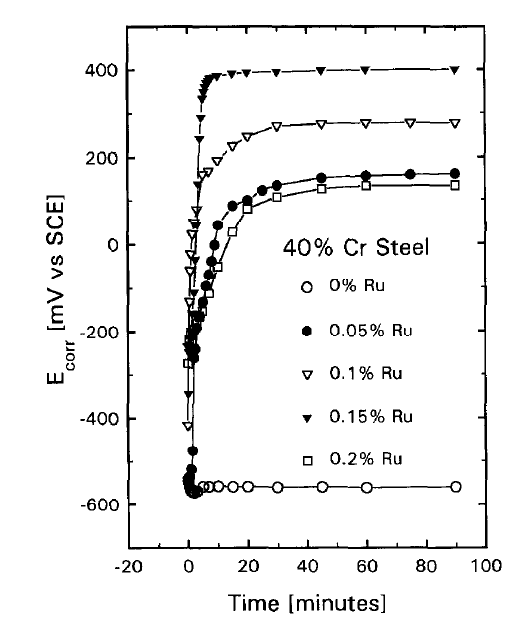
\includegraphics[width=.95\linewidth]{chapters/austenitic_steels_in_nuclear/images/fe40crru.png}
\end{minipage}
\caption{Addition of Ru to Fe30Cr and Fe40Cr steels - open current corrosion potential variation with time in 10\% sulphuric acid\cite{potgieter1994}}
\label{fig:ruadditions}
\end{figure}

It was found that an addition of 0.15\% \Gls{Ru} (out of a selection of 0\%, 0.05\%, 0.10\%, 0.15\% and 0.20\%) was optimum for both Fe30Cr and Fe40Cr steel (fig. \ref{fig:ruadditions})\cite{potgieter1994}.  Other \acrshort{pgm}s may be used for cathodic modification, including \Gls{Pd}, \Gls{Ir} and \Gls{Pt}, but the cost of the metal must be weighed against the possible gains.

\begin{figure}
\centering
\begin{minipage}{.50\textwidth}
\centering
    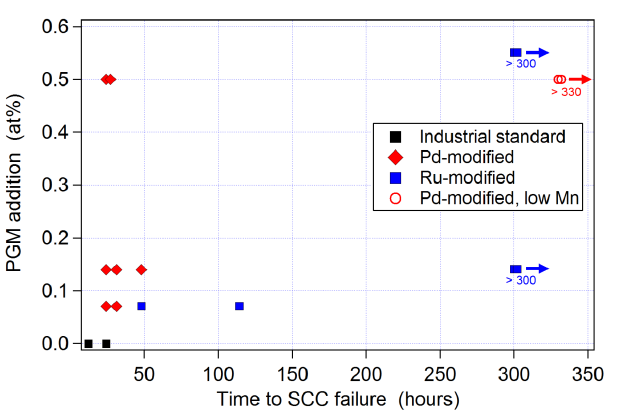
\includegraphics[width=.99\linewidth]{chapters/austenitic_steels_in_nuclear/images/pgmfailure.png}
    \caption{Failure times for 304SS, Pd doped 304SS (with and without Mn) and Ru doped 304SS in polythionic acid at ambient temperature\cite{scrstainless}}
    \label{fig:pgmfailuretimes}
\end{minipage}
\end{figure}

Connolly et al recently added Ru and Pd to \gls{304SS} samples that were sensitized at 920K for 24 hours\cite{scrstainless}.  After sensitization, the steel was analysed by \acrshort{tem} and Cr-rich carbides were found at grain boundaries.  Without the passive protection due to Cr, the samples were exposed to polythionic acid to promote \acrshort{scc}.  The Ru doped steels performed well, but the Pd doped steels showed no improvement over regular 304SS.  Further analysis of the samples by \acrshort{tem} reveals that the low percentage of Mn in the steel allows the formation of Pd-Mn precipitates at the grain boundary\cite{scrstainless}.  These precipitates form during the sensitization procedure and thus negate the protection by cathodic modification at the surface of the metal by removing the Pd.

With a low Mn 304SS (less than 0.05\% Mn), varied amounts of Pd have been tested.  With the reduction in Mn the corrosion resistance improves greatly over regular 304SS.  Palladium remains at the surface, as the amount of Mn is too low for appreciable amounts of Pd to be lost to precipitate formation during sensitization.  No failures have been observed with either the Ru or Pd (low Mn) samples for 330 hours exposure to polythionic acid at ambient temperatures (fig. \ref{fig:pgmfailuretimes}) \cite{scrstainless}.

The surface of the metal does not need to have a full coating of \acrshort{pgm} but it should be equally spaced across the surface.  Oxidant in the layer at the surface will be consumed at the locations of \acrshort{pgm}s and the change in concentration at those points will naturally cause diffusion of more oxidant to those locations\cite{noblemetalchemical}.

The \acrshort{pgm}s may be coated on the surface of the metal or alloyed to the metal.  The first method is the more cost efficient but if a crack does form, or if a layer is removed, it will expose the regular alloy underneath.  If the \acrshort{pgm} is alloyed, there will always be protection, unless a mechanism is removing the \acrshort{pgm} from the surface.  This could be through precipitation as a carbide, or it could be due to radiation causing the metals to segregate.

\begin{table}[h]
\begin{center}
\renewcommand{\arraystretch}{1.2}
\begin{tabular}{c c}
\hline\hline
Reaction & Product Halflife\\
\hline\hline
${}^{54}Cr(n, \gamma){}^{55}Cr$ & 3.5 mins \\ 
${}^{64}Ni(n, \gamma){}^{65}Ni$ & 2.5 hrs  \\
${}^{55}Mn(n, \gamma){}^{55}Mn$ & 2.6 hrs  \\
${}^{104}Ru(n, \gamma){}^{105}Ru$ & 4.4 hrs  \\
${}^{108}Pd(n, \gamma){}^{109}Pd$ & 13.7 hrs  \\
${}^{196}Pt(n, \gamma){}^{197}Pt$ & 19.9 hrs  \\
\hline\hline
\end{tabular}
\end{center}
\caption{Radioactive products and their half lives for \acrshort{pgm} doped 304SS}
\label{table:304ssradioactive}
\end{table}

Adding elements to metals, even in small amounts, may be problematic as certain elements have high neutron reaction cross sections and transmute into radioactive isotopes.  ${}^{55}Cr$ is a concern for all neutron irradiated stainless steels, but with a very short half life it quickly cools and becomes less of a concern, with ${}^{65}Ni$ becoming the dominant source of activity after 10 hours.  Adding Mn to steel that is in a reactor is known to result in an increase in activity due to the ${}^{55}Mn(n, \gamma){}^{56}Mn$ reaction (section \ref{section:effectsofradiationorg}).  

The addition of \acrshort{pgm}s alters the activity of the steel following neutron irradiation and with just a 1\% addition there is an increase in activity comparable to that of the 10\% Ni transmuted to ${}^{65}Ni$.  This is due to reactions that create ${}^{105}Ru$, 
 ${}^{109}Pd$ and ${}^{197}Pt$ for Ru, Pd and Pt respectively (table \ref{table:304ssradioactive}).  

With such small additions required for cathodic modification and the short half lives of the radioactive isotopes, there isn't a concern due to neutron activation over regular 304SS, and much less of a concern than that of 304SS containing Mn. More data computed using the \acrshort{tendl} library is available in appendix \ref{section:pgmactivity}.





